\documentclass{gescons}

\genre {Entrevista}
\author{Roberta Bouchardet}
\title{Interassistência: Teoria e~Prática Sob a~Ótica da Conscienciologia}
\paginaurl{https://www.youtube.com/live/zasm7A2swDQ}

\begin{document}
    \makeentrevistatitle
    \coverart{back/Roberta_Bouchardet}
    \vspace*{\fill}

    \begin{multicols}{2}

\begin{center}
    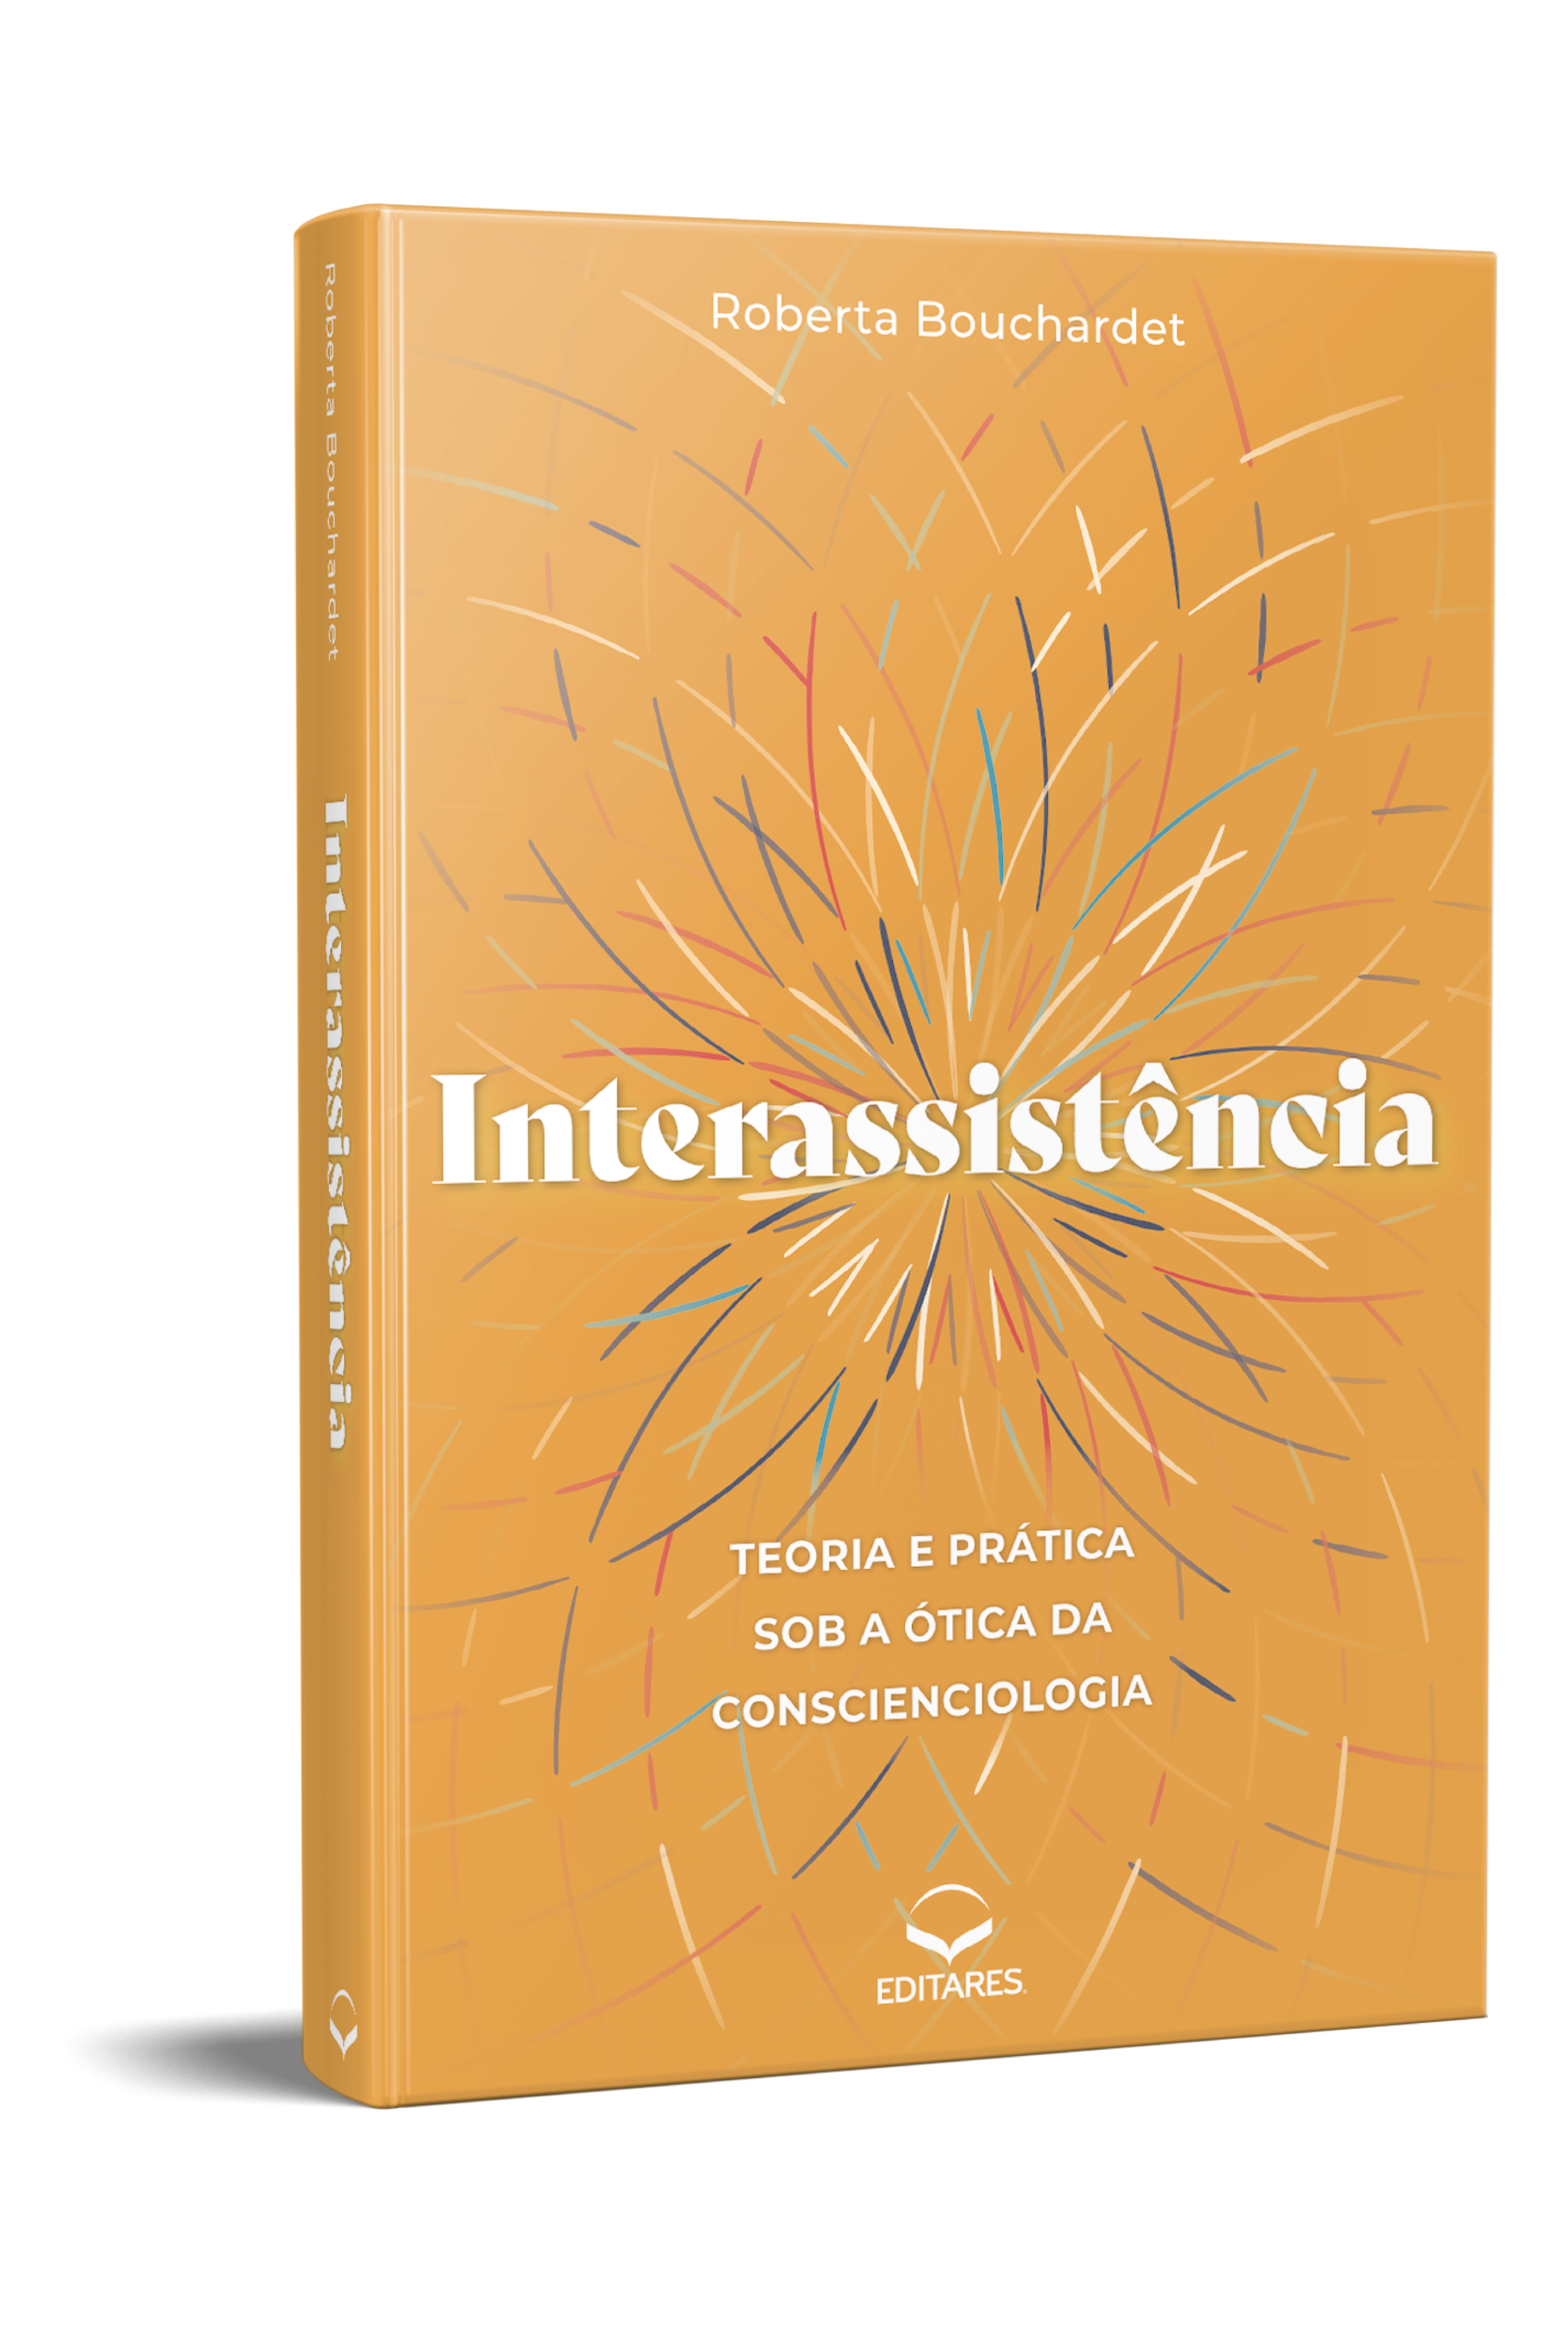
\includegraphics[width=7cm]{articles/entrevista/mockups/Roberta-Bouchardet}
\end{center}

%\begin{center}
%    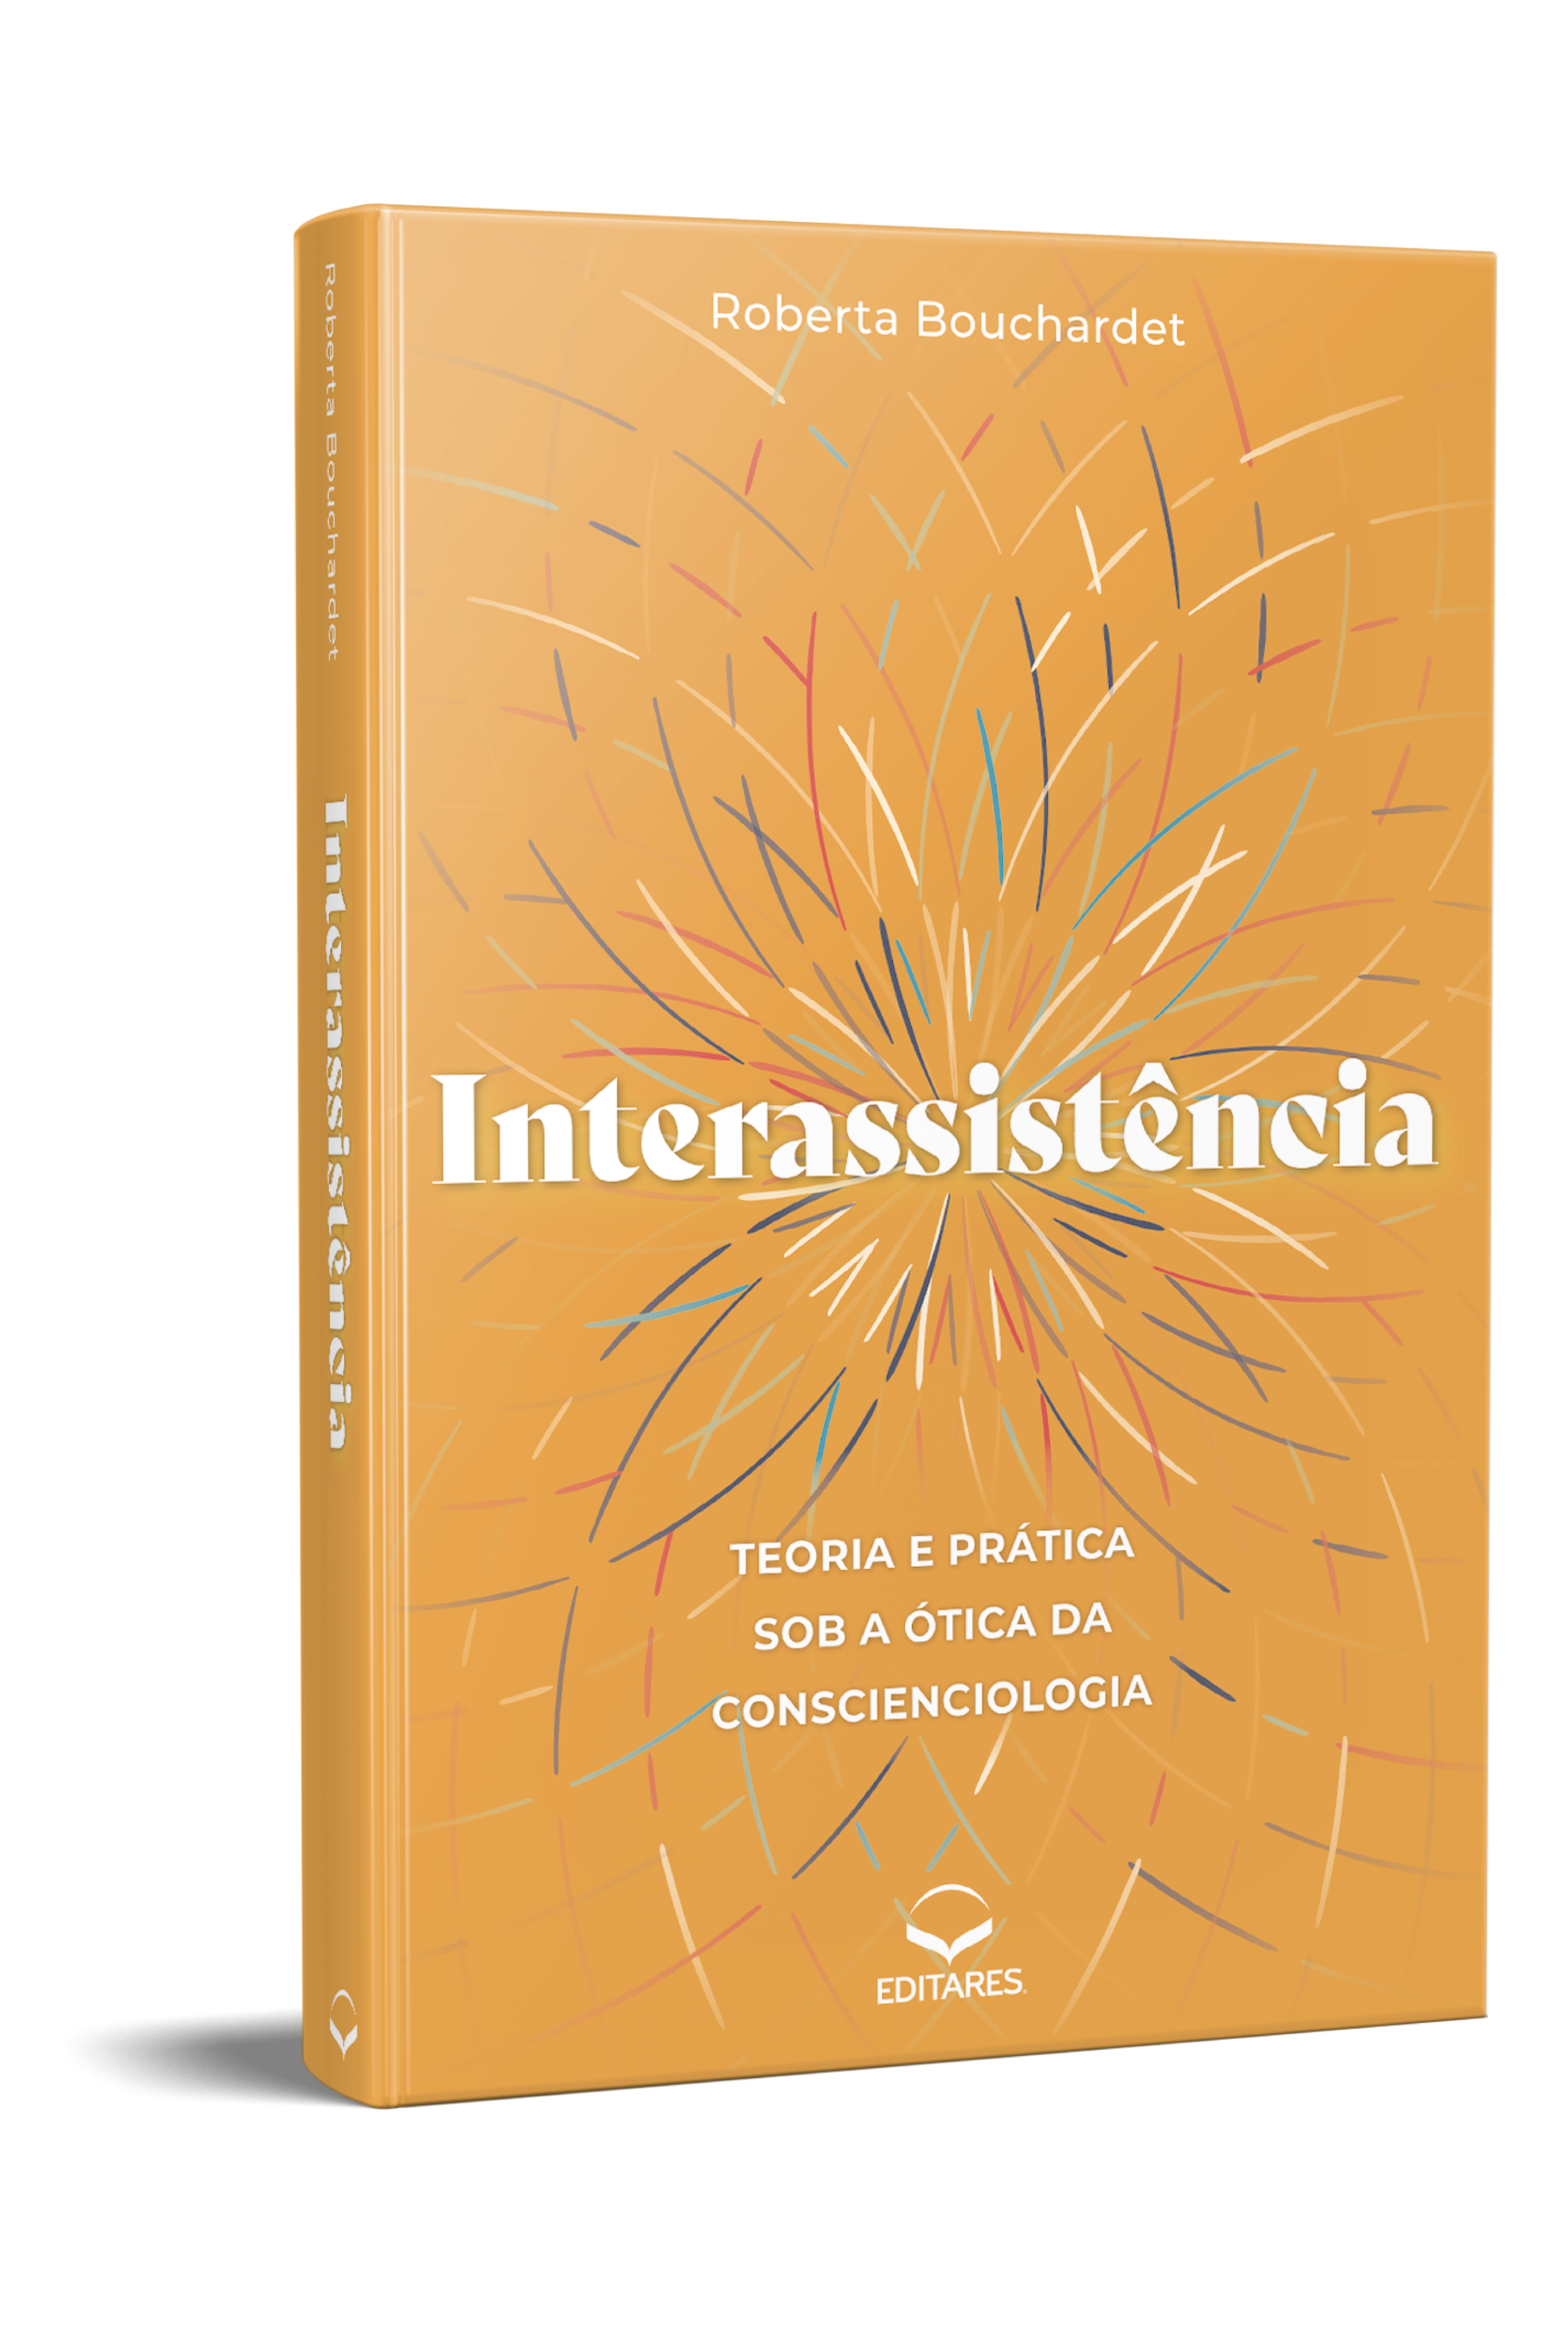
\includegraphics[width=8cm]{articles/entrevista/mockups/Roberta-Bouchardet}
%\end{center}

\textbf{1.       Qual foi a~motivação para a~escrita da obra? Por que a~definição deste tema para publicação de um livro?}

Sempre gostei de livros e~de escrever. E~assim, junto com o~incentivo do Prof. Waldo em deixar uma gestação consciencial nessa existência, veio a~motivação de registrar parte do conhecimento adquirido em tantas décadas de estudo e~autopesquisas na Conscienciologia. A~definição do tema veio aos poucos. Começou com o~verbete Autoamparo, que deveria ser a~base do livro, mas a~temática cresceu e~se tornou Interassistência, sendo o~Autoamparo um dos capítulos do livro.

\textbf{2.       Quais foram as principais percepções, intra e~extrafísicas, durante a~pesquisa e~a~escrita da obra? E~posterior ao lançamento?}

Já há alguns anos eu estava escrevendo alguns capítulos, sem saber ainda o~escopo da obra, e~no Acoplamentarium de pesquisa, durante uma prática energética, tive o~fenômeno de captação de ideias e~visualizei todo o~sumário, os capítulos a~serem escritos. Anotei tudo e~a~partir daí a~escrita fluiu bem mais rapidamente. Durante a~escrita, sentia-me muito motivada e~energizada, o~mentalsoma não cansava. O~que cansava era o~soma, que exigia parar. Após o~lançamento, percebo mudanças pensênicas, maior tranquilidade, talvez novos amparadores, o~que está em avaliação ainda.

\begin{pullquote}
    ``Durante a~escrita, me sentia muito~motivada e~energizada, o~mentalsoma não cansava''
\end{pullquote}


\textbf{3.       Qual o~maior aprendizado com a~escrita desta obra?}

Aprendi muito sobre o~processo de organização de uma obra para publicação. Uma coisa é~escrever textos para nós mesmos ou trabalhos para cursos. Outra, muito diferente, é~o~livro. Muitas etapas são necessárias e~muitas pessoas são envolvidas e~trabalham arduamente junto com o~autor. Durante o~processo, tornei-me participante do Conselho Editorial da Editares e~busco auxiliar outros autores nesse processo. É~preciso persistência e~paciência; a~pressa em fazer rápido acaba assediando o~fluxo e~atrasando mais ainda os trabalhos. É~preciso trabalhar ombro a~ombro, tanto com os amparadores extrafísicos, como também com os colegas intrafísicos nas várias etapas de edição do livro. Entrar em conflito é~contraproducente.

\begin{pullquote}
    ``É preciso persistência e~paciência; a~pressa em fazer rápido acaba assediando o~fluxo e~atrasando mais ainda os trabalhos.''
\end{pullquote}

\textbf{4.       O~que poderia dizer como incentivo para que mais pesquisadores invistam na publicação de obras conscienciológicas?}

Escolha uma temática de interesse, busque bibliografia em todas as bases de consulta da Conscienciologia e~comece a~focar naquele assunto. Busque convergir as atividades para aquela temática, anote as experiências. Antes de começar a~escrever, defina o~escopo, a~estrutura do livro e~o~público-alvo. E~busque assessoria da Uniescon. Há várias atividades na IC para ajudar o~autorando. 
    
    
    \end{multicols}
    \vspace*{\fill}
\end{document}
